% The option 11pt uses 11-point font size.  You can use 12pt if you like.
% The documentclass amsart stands for "AMS article".
% The AMS is the American Mathematical Society.  Join it for magazines and other benefits.

\documentclass[11pt]{amsart}

% Geoemtry is a cool package.  It allows you to set page size and layout options.
\usepackage{geometry}                
\geometry{letterpaper}                   

% Below are a bunch of pictures for making graphics, special symbols, diagrams, web-links, and more.
\usepackage{graphicx}
\usepackage{accents}
\usepackage{amsfonts}
\usepackage{amscd}
\usepackage{amssymb}
\usepackage{stmaryrd}
\usepackage{hyperref}
\usepackage{url}
\usepackage{tikz}
\usetikzlibrary{shapes}
\usepackage{multirow}
\usepackage{fullpage}
\usepackage{amsthm}
\usepackage{color}
\usepackage{url}
\usepackage[]{mdframed}

\newcommand{\bracket}[1]{\langle #1 \rangle}

% Here are some commands that I like to use often.
% For example, typing \NN will make a "blackboard bold" N, standing for the natural numbers.
% The command \newcommand makes a new command.
% The code \mathbb stands for "math blackboard bold" font.
\newcommand{\NN}{{\mathbb N}}
\newcommand{\ZZ}{{\mathbb Z}}
\newcommand{\QQ}{{\mathbb Q}}
\newcommand{\RR}{{\mathbb R}}
\newcommand{\CC}{{\mathbb C}}

%Here are some commands to make theorems, corollaries, lemmas, remarks, and definitions.
\newtheorem{thm}{Theorem}%[section]   %Uncomment the [section] if you want theorems numbered like Theorem 1.1.
\newtheorem{cor}[thm]{Corollary}
\newtheorem{lem}[thm]{Lemma}
\theoremstyle{remark}
\newtheorem{rem}[thm]{Remark}
\theoremstyle{definition}
\newtheorem{defn}[thm]{Definition}

\title{A Short Paper}
\author{Eli Hantman}
\date{}                                           % Activate to display a given date or no date

\begin{document}
\maketitle

I think LaTex is                  pretty cool!  
%Everything after a percent sign is a comment.
%You can see comments in your text editor, but they will not appear in the compiled document.
%I'll use comments to describe how LaTex works here.
%Notice that space doesn't compile to space in LaTex.  I put lots of empty space between "is" and "pretty", but only one space shows up in the compiled document.
%The idea is to *trust LaTex* to make the spacing right.
Instead of using some silly equation editor, I just type little codes and LaTex makes it look pretty and professional.  For example, $\int_{-\infty}^\infty e^{-x^2} dx = \sqrt{\pi}$.
%DO use dollar sounds around all mathematical expressions.  The mathematical expression x^2 + 3 is between single dollar-signs above, so LaTex will make it look really pretty.
%Just about every LaTex command begins with a backslash.
%The LaTex command \int makes an integral sign.
%The underscore "_" puts in a subscript.
%The LaTex command \infty makes the infinity symbol.
%Notice that -\infty is contained in braces {...} -- that makes LaTex put the entire "negative infinity" in the subscript of the integral.
%The caret "^" puts in a superscript (exponent).
%Notice that braces aren't necessary around the \infty.  One command doesn't need to be grouped.
%The \sqrt{...} command puts things under a square root sign.  
%The \pi command makes... a pi.
Big and important equations deserve their own line.  For this, I use double-dollar signs around the math.  And here it goes!
%The difference between one empty line, two empty lines, or 15 empty lines is nothing.
%But one empty line does have an effect:  it causes a paragraph break.  Look at the indentation in the compiled document.
%Each new paragraph is indented.  Don't indent in your Tex file!  No tabs!
$$\sqrt{1 + \sqrt{1 + \sqrt{1}}} = \sqrt{1 + \sqrt{2}}.
$$
%Use double dollar signs, and LaTex will put the math on it's own line, centered.
Sometimes, I like to put equations line after line after line.  
\begin{align*}
    x &= x + 1 - 1 \\
      &= x + 1 - 1 + 1 - 1 \\
      &= x + 1 - 1 + 1 - 1 + 1 - 1.
\end{align*}
%Environments begin with a \begin{...} and end with an \end{...}
%Above, there is an "align*" environment.  
%This environment is for multiple lines of mathematics, with alignment controlled by the ampersand (&) character.
% In each line, the &= will be lined up above the &= in the next line.
%Use double backslashes, \\, to start the next line in the environment.
%The * at the end of "align" tells LaTex *not* to number the equation.  Try getting rid of the * and see what happens!

We use special symbols for the sets of natural numbers, integers, rational numbers, real numbers complex numbers, quaternions, and octonians.  $\NN \subset \ZZ \subset \QQ \subset \RR \subset \CC\subset \mathbb H\subset \mathbb O$. You can write down any equations. There are many manuals of LaTeX you can consult with. Some of these are listed in Module tab of Math 100 Canvas page. 

I can even draw pictures in LaTex using the TikZ/PGF package!

\begin{center}
    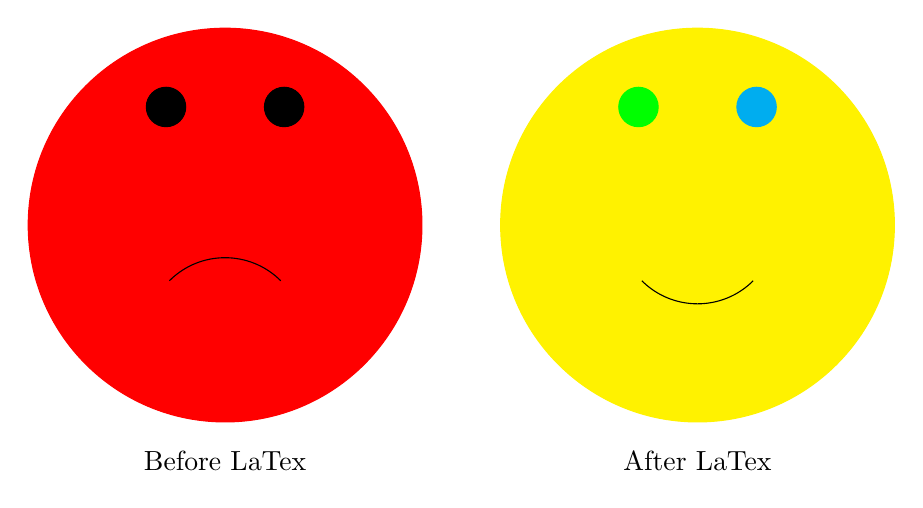
\begin{tikzpicture}[scale=0.5]
        \filldraw[red] (0,0) circle (5);
        \filldraw[black] (-1.5,3) circle (0.5);
        \filldraw[black] (1.5,3) circle (0.5);
        \draw (-135:2) arc (135:45:2);
        \draw (0,-6) node {Before LaTex};
        \begin{scope}[xshift=12cm]
            \filldraw[yellow] (0,0) circle (5);
            \filldraw[green] (-1.5,3) circle (0.5);
            \filldraw[cyan] (1.5,3) circle (0.5);
            \draw (-135:2) arc (-135:-45:2);
            \draw (0,-6) node {After LaTex};
        \end{scope}
    \end{tikzpicture}
\end{center}
%Here I've used an environment inside an environment.
%The "center" environment does the obvious thing -- it centers whatever's inside of it.
%The "tikzpicture" environment starts a picture, using the "TikZ/PGF package" for drawing commands.
%TikZ/PGF is complicated and powerful.  We'll learn more later!

You can see more examples of TikZ and PGF at \url{http://www.texample.net/tikz/} Just search for TikZ, and you will get more introductory examples. 
%By putting a full URL (web address) within the \url{...} command, LaTeX will put it into a computer-style font, and make it clickable in a PDF file.  
Read more about LaTeX by looking at Gratzer's book\cite{Gratzer}.
%Refer to a citation with the \cite command.  Within the braces is the "key" -- here the "key" is Gratzer.
%LaTeX will insert a numbered link to the citation.


\pagebreak
\section{Some cool Theorems}

A theorem I quite like is known as the Separating Axis Theorem (SAT),
which is a special case of the Separating Hyperplane Theorem. It is
commonly used in Physics simulation since it simplifies the
logic.

Here is a proof of the Separating Hyperplane Theorem from
Wikipedia.

\begin{thm}
    \begin{mdframed}
        Let A and B be two disjoint nonempty convex subsets
        of $\mathbb{R}^n$. Then there exist a nonzero vector
        $v$ and a real number $c$ such that:

        \begin{gather}
            \bracket{x, v} \ge c \text{ and } \bracket{y, v} \le c
        \end{gather}

        For all $x \in A$ and $y \in B$.

        If both sets are closed and at least one is compact,
        then the separation can be strict, that is:

        \begin{gather}
            \bracket{x, v} > c \text{ and } \bracket{y, v} < c
        \end{gather}

        \begin{mdframed}
            \begin{rem}
                It should be noted that $\bracket{a, b}$ denotes the
                inner product. In common applications to linear algebra
                and geometry this would be the dot product, but it
                had the property of taking in $a, b \in \mathbb{R}^n$
                and mapping them to some value $c \in \mathbb{R}$.
            \end{rem}
        \end{mdframed}
        \vspace{8pt}

        Assume $A$ and $B$ to be disjoint, nonempty, and convex subsets
        of $\mathbb{R}^n$. The summary is as follows:

        \begin{center}
            \begin{tabular}{|c|c|c|c|}
                \hline
                A & B & $\bracket{x, v}$ & $\bracket{y, v}$\\ 
                \hline
                  &   & $\ge c$ & $\le c$\\
                  \hline
                closed compact & closed & $>c_1$ & $< c_2 \text{ with } c_2 < c_1$\\
                \hline
                closed & closed compact & $> c_1$& $< c_2 \text{ with } c_2 < c_1$\\
                \hline
                open & & $>c$ & $\le c$\\
                \hline
                open & open & $>c$ & $<c$\\
                \hline
            \end{tabular}
        \end{center}

        The number of dimensions must also be finite. If the sets are compact
        then it is possible to generalize to infinite dimensions, which is known
        as the Hahn-Banach separation theorem.
    \end{mdframed}
\end{thm}

\begin{lem}
    Let $A$ and $B$ be two disjoint closed subsets of $\mathbb{R}^n$,
    and assume $A$ is compact. Then there exists points $a_0 \in A$
    and $b_0 \in B$ minimizing the distance $||a - b||$ over
    $a \in A$ and $b \in B$.
\end{lem}

Proof of Lemma 2:
\vspace{8pt}
\begin{mdframed}
    Let $a \in A$ and $b \in B$ be any pair of points, and let
    $r_1 = ||b - a||$. Since $A$ is compact, it is contained
    in some ball centered on $a$; let the radius of this ball
    be $r_2$.

    Let $S = B \cap \overline{B_{r_1 + r_2}(a)}$ be the intersection
    of $B$ with a closed ball of radius $r_1 + r_2$ centered around
    $a$.

    Then $S$ is compact and nonempty because it contains $b$. Since
    the distance function is continuous, there exist points
    $a_0$ and $b_0$ whose distance $||a_0 - b_0||$ is the minimum
    over all pairs of points in $A \times S$.

    To prove that $a_0$ and $b_0$ have the minimum distance over all
    pairs of points $A \times B$. Suppose that there exists points
    $a'$ and $b'$ such that $||a' - b'|| < ||a_0 - b_0||$. Then in
    particular $||a' - b'|| < r_1$, and by the triangle inequality,
    $||a - b'|| \le ||a' - b'|| + ||a - a'|| < r_1 + r_2$. 

    Therefore $b'$ is contained in $S$, which contradicts the
    fact that $a_0$ and $b_0$ had minimum distance over $A \times S$.\qed
\end{mdframed}

\pagebreak
Proof of Theorem:

\vspace{8pt}
\begin{mdframed}
    We first prove the second case.

    Without loss of generality, $A$ is compact. By the lemma,
    there exist points $a_0 \in A$ and $b_0 \in B$ of minimum
    distance to each other. Since $A$ and $B$ are disjoint,
    we have $a_0 \neq b_0$. Now, construct two hyperplanes
    $L_A$,$L_B$ perpendicular to the line segment $[a_0, b_0]$,
    with $L_A$ across $a_0$ and $L_B$ across $b_0$. We claim,
    neither $A$ nor $B$ enters the space between
    $L_A$, $L_B$, and thus the perpendicular hyperplanes to
    $(a_0, b_0)$ satisfy the requirement of the theorem.

    Algebraically, the hyperpanes $L_A$ and $L_B$ are defined by
    the vector $v := b_0 - a_0$, and the two constants
    $c_A := \bracket{v, a_0} < c_B := \bracket{v, b_0}$, such that
    $L_A = \{x : \bracket{v, x} = c_A \}$, $L_B = \{x \bracket{v, x} = c_B \}$.
    Our claim is that $\forall a \in A, \bracket{v, a} \le c_A$ and
    $\forall b \in B, \bracket{v, b} \ge c_B$.

    Suppose that $a \in A$ such that $\bracket{v, a} > c_a$, then
    let $a'$ be the foot of perpendicular from $b_0$ to the line
    segment $[a_0, a]$. Since $A$ is convex, $a'$ is inside $A$,
    and by planar geometry, $a'$ is closer to $b_0$ than $a_0$,
    contradiction.

    Similar arguements apply to $B$.

    \vspace{20pt}

    For the first case,

    Approach both $A$,$B$, from the inside by $A_1 \subseteq A_2 \subseteq ...
    \subseteq A$ and $B_1 \subseteq B_2 \subseteq ... \subseteq B$.
    such that $A_k$,$B_k$ is closed and compact, and the unions are the
    relative interiors $relint(A)$, $relint(B)$.

    \begin{mdframed}
        \begin{rem}
            I am somewhat unfamiliar with the relative interior. Apparently
            it is a generalization of the interior which allows low dimensional
            sets in high dimensional spaces to have meaningful interiors.
        \end{rem}
    \end{mdframed}

    Now by the second case, for each pair $A_k$, $B_k$ there
    exists some unit vector $v_k$ and real number $c_k$ such that
    $\bracket{v_k, A_k} < c_k < \bracket{v_k, B_k}$.

    Since the unit sphere is compact, we can take a convergent
    subsequence, so that $v_k \to v$. Let
    $c_A := {sup}_{a \in A}\bracket{v, a}$, $c_B :=
    {inf}_{b \in B}\bracket{v, b}$. thus separating $A$ and $B$.

    Assume not, then there exists some $a \in A$, $b \in B$
    such that $\bracket{v, a} > \bracket{v, b}$, then since
    $v_k \to v$ for large enough $k$, we have
    $\bracket{v_k, a} > \bracket{v_k, b}$, contradiction.

\end{mdframed}
\vspace{8pt}

There is more proof for each case as well as specific properties
of each case however I think this illustrates the core
theorem.


Generally in simulations the property that if two convex,
compact sets are disjoint there must exist some projection
in which they are disjoint is used. However in recent
years this method has been superseeded by the Gilbert-Johnson-Keeli
algorithm which has a better algorithmic performance for
3 dimensions and high complexity sets.

\begin{thebibliography}{1}
\bibitem{Gratzer} G. Gr\"atzer, ``More Math Into LaTeX, 4th Edition,'' Springer 2007.
\bibitem{Wiki} ``Hyperplane Separation Theorem,`` Wikipedia
\end{thebibliography}
%Here we include a short bibliography, with one source.
%Each source is a "bibitem".  The command \bibitem{KEY} makes a bibliography item, with key KEY.
%We used the key "Gratzer" so we can use the command \cite{Gratzer} anywhere within the file to cite it.
%Notice the command \"a put an accent (two dots) over the "a" in Gratzer's name.
%LaTeX does not like double-quotes.  To put the book title "More Math Into LaTeX" into quotes,
%you must use two single-back-quotes `` to open the quote,
%and two single-forward-quotes ' ' to close the quote.  It is annoying, I think.
%LaTeX automatically numbers the bibitems.
%In this basic mode, you are in charge of formatting and ordering your bibliography.
%Using BibTeX, these steps can be simplified.

\end{document}  
%The \end{document} command ends the document.
%Anything written after \end{document} will be ignored.

Ignore me!
